\documentclass[14pt]{article}
\usepackage{url, hyperref}
\usepackage[margin=1in]{geometry}
\usepackage{xcolor}
\usepackage{listings}
\usepackage{graphicx}

\lstdefinelanguage{JavaScript}{
  morekeywords={typeof, new, true, false, catch, function, return, null, catch, switch, var, if, in, while, do, else, case, break},
  morecomment=[s]{/*}{*/},
  morecomment=[l]//,
  morestring=[b]",
  morestring=[b]'
}

\linespread{1.2}
\renewcommand{\contentsname}{Table of Contents}
\newcommand{\codeword}{\texttt}

\title{Developing a Browser Extension for SEO Analysis and Report Generation}
\author{
  \\[142pt]
  CS252 Project Report \\
  Presented to\\
  Dr. Thomas Austin\\
  Department of Computer Science \\
  San Jos\'{e} State University \\
  Fall 2017
  \bigskip
  \\[142pt]
  By\\
  Vikram Deshmukh \\
  }

\begin{document}
\bigskip


\maketitle
 
\pagebreak


\begin{abstract}
\normalsize{
Search Engine Optimization (SEO) has become an integral part of publishing any content on the web. The primary goal of SEO is to ensure higher visibility to the content. It is imperative to perform SEO on any web-related content that one wishes to make index-able by search engines. The main goal of this project was to develop a browser extension that performs SEO analysis and displays a report within the browser without requiring the user to leave the page.


Due to it's convenience and extremely lucid documentation, Chrome was the browser of choice for developing this extension.


\textit{\textbf{Key Items}\textemdash Search Engine Optimization, Chrome, Extension, TypeScript, ECMAScript6, Singleton}
}
\end{abstract}

\smallskip

\pagebreak
\tableofcontents
\pagebreak
\section{Introduction}
Search Engine Optimization (SEO) is an important step when it comes to authoring content for the web. There are many tools and small organizations that are dedicated to performing SEO analysis of existing sites and making suggestions to improve content visibility. There are also some existing extensions in the Chrome Web Store and Firefox Add-ons Gallery. But these are either marred by bad reviews due to functionality issues or charge their users for premium access. The goal of this project is to develop an extension that perform SEO analysis and generates a report within the browser.

\subsection{Importance of performing SEO}
It is imperative nowadays to have any content on the web optimized for search engines. Some of the biggest benefits of ensuring that web pages are search engine optimized are summarized below ~\cite{seo}:

\begin{itemize}
    \item Higher Page Rank
    \item Increases visibility
    \item Increases frequency of appearing in search results
    \item Increased website traffic (thereby revenue)
\end{itemize}


The process of SEO primarily involves of 2 actions:

\subsection{Content Optimization}
Content Optimization involves enhancing the quality of the content on the webpage by including internet buzz words like \textit{Free}, \textit{Online}, \textit{Download} while also ensuring that most relevant keywords appear frequently and strategically throughout the page content. This ensures that the search engines give higher ranking to your page when any users search for those particular keywords.

\smallskip

\subsection{Markup Optimization}
Markup Optimization, unlike content optimization, has nothing to do with the content on the page. In fact, it is also about the syntactic details about how the page has been constructed. With the advent of HTML5, web developers can afford to indulge themselves in creating a webpage that uses newer tags that are semantically relevant while also adding some syntaxing sugar. For example, \textit{header}, \textit{footer}, \textit{aside}, \textit{video}, etc. Search engines tend to prefer web pages that adhere to the newer HTML specification.
\smallskip


\section{Requirement Gathering}
The very first step involved gathering information about SEO guidelines, processes, and understanding how various search engines parse web pages. This step also involved understanding the best practices, dos and donts of SEO in order to come up with a rubric to evaluate any given web page. This information was critical as it would be later used to create a rubric for evaluation of the web page.

\subsection{The Rubric}
After reading through Google SEO Guidelines ~\cite{googleSEO} and SEO Analytics and Reporting section on Moz.com ~\cite{mozSEO}, here is the rubric that was created:

\begin{itemize}
\item{Presence of exactly one \codeword{H1} tag}
\item{Missing meta tags like \codeword{description}, \codeword{keywords}, etc.}
\item{Presence of broken links}
\item{Page Redirect, if any, should be HTTP status 301 (Server-side redirect)}
\item{Missing closing tags}
\item{\codeword{img} tags with empty or missing \codeword{alt} attribute}
\item{Empty tags in the document}
\item{\codeword{description} or \codeword{title} too long/short}
\end{itemize}

After testing the document markup against this rubric, any problem encountered with the markup is classified as \textit{Critical}, \textit{Important}, \textit{recommended}. The page is then given an overall rating in the form of a smiley face: sad, neutral, or happy.


\smallskip

\section{Implementation}
Being an extension for the Chrome browser ~\cite{gExt}, opting for JavaScript was the obvious choice. But as we had seen during the Intro to JavaScript class ~\cite{lectureslides}, there are many ways of declaring a class and writing Object Oriented code in JavaScript with their own pros and cons. So, it was decided to use TypeScript to write clean, type-safe JavaScript. 

The steps involved are mentioned below:

\begin{enumerate}
  \item Read Page Source.
  \item Sanitize HTML: Remove comments, scripts tags and inline scripts, link and style tags using the \codeword{HTMLSanitizer.js} file.
  \item Analyze HTML against the rubric using the \codeword{HTMLAnalyzer.js} file.
  \item Display the results of analysis in the extension window.
\end{enumerate}

I decided to write HTML String sanitizer code and code that performs SEO analysis as reusable, independent libraries. Also, in order make these truly reusable, the libraries are written using the Singleton pattern to ensure only a single instance of the library is available to the developer for use.

Since there may be instances when a non-tech person needs to share the generated report with the developer so that the developer can fix the reported errors, there is also a feature for downloading the generated report as a PDF file. This nifty little feature was adding using an existing jqPDF library ~\cite{jqPDF}.

Given below is a code snippet that shows how Singleton classes in created using TypeScript and the resulting JavaScript.

\begin{lstlisting}[language=JavaScript, caption={TypeScript code for singleton pattern},captionpos=b, xleftmargin=.1\textwidth]

//  TypeScript
namespace HTMLAnalyzer {
    export function analyze(str: string) { … }
}

//  JavaScript version with closure
var HTMLAnalyzer;
(function (HTMLAnalyzer) {
    function analyze(str) { … }
    HTMLAnalyzer.analyze = analyze;
})(HTMLAnalyzer || (HTMLAnalyzer = {}));

\end{lstlisting}
\smallskip
\smallskip

Here's a screenshot of the extension in action when triggered on a simple HTML page without an \codeword{title} or \codeword{meta} tags and with only a few hyperlinks.

\begin{figure}[!ht]
\centering
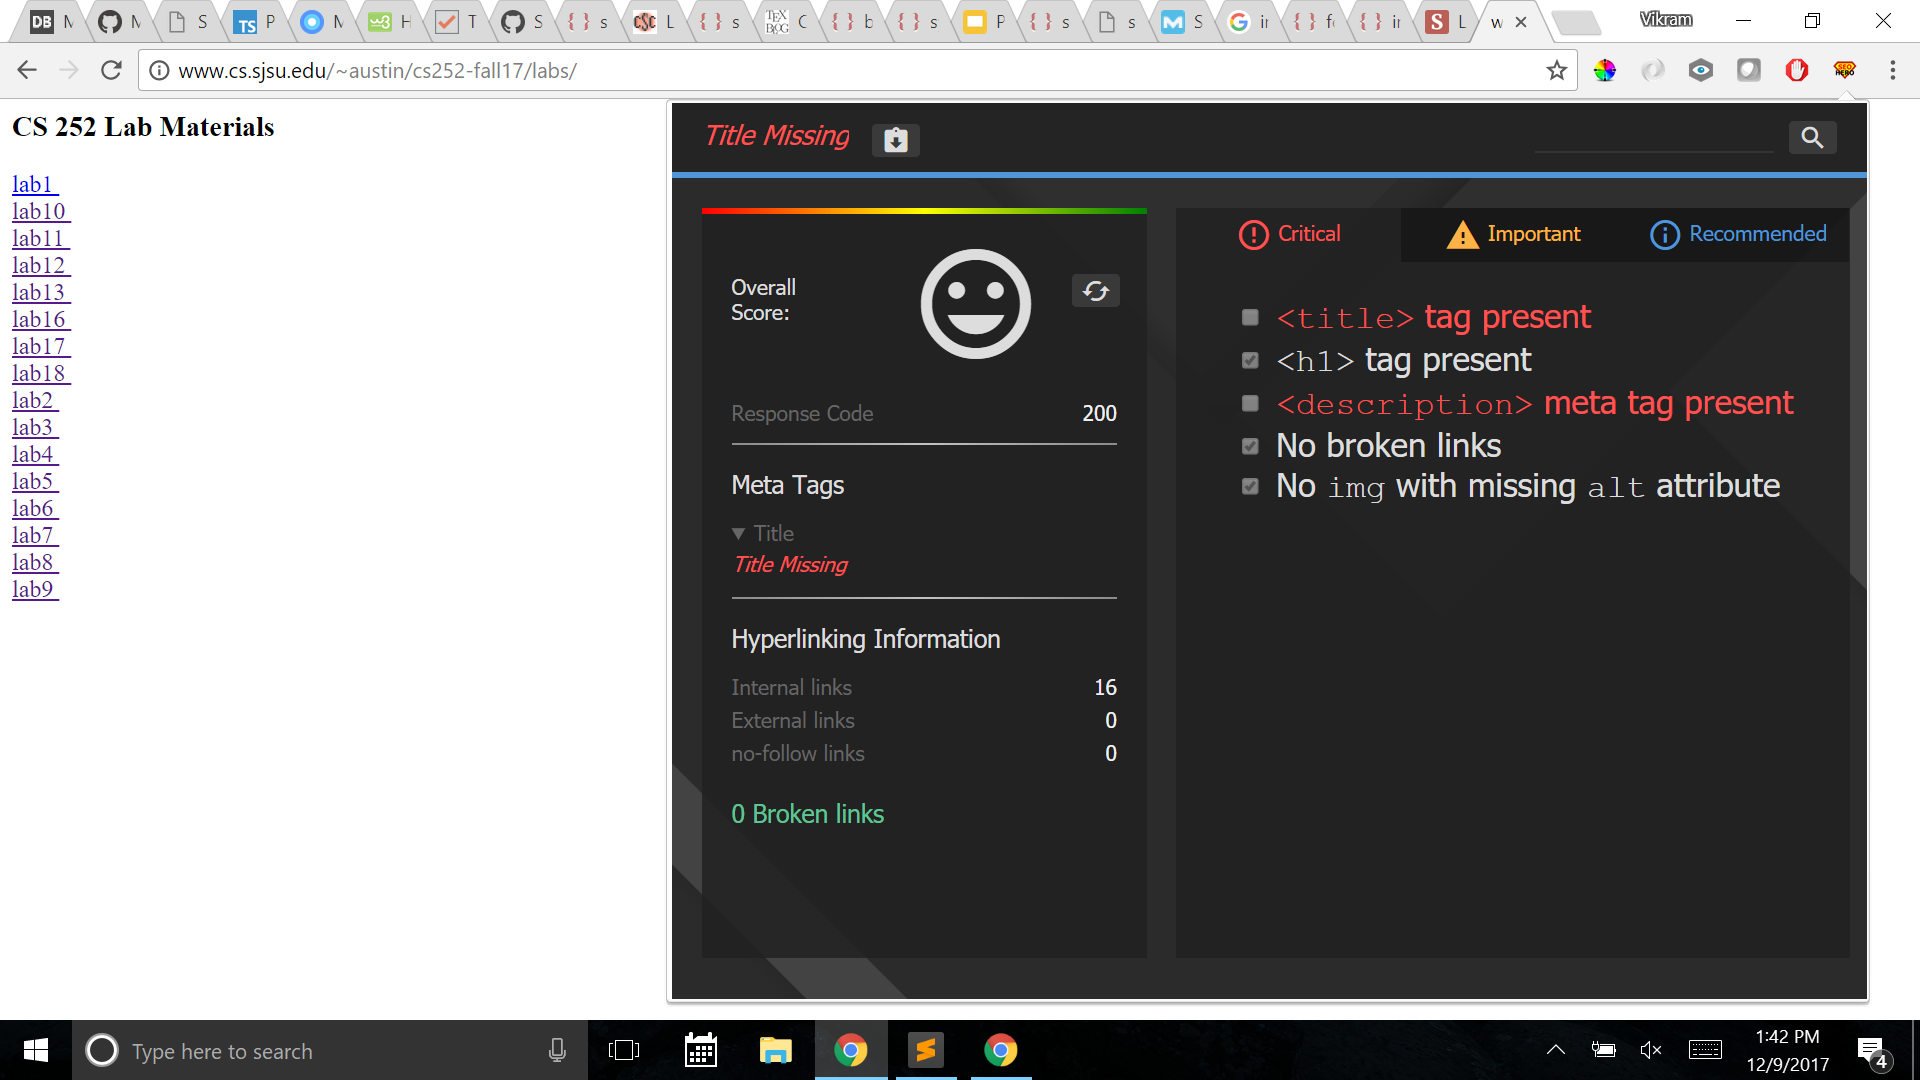
\includegraphics[scale=0.22]{Screenshot}
\caption{Screenshot of the extension in action}
\end{figure}


\smallskip

\section{Deployment}
Deploying to Chrome Web Store is an extremely simple and easy process. To publish your app to the Chrome Web Store, follow these steps ~\cite{publishing}:

\begin{enumerate}
  \item{Create your app zip file}
  \item{Create a developer account}
  \item{Upload your app}
  \item{Get app constraints (like app ID, OAuth token) and finish your app code}
  \item{Pay the developer signup fee}
  \item{Publish your app}
\end{enumerate}

Once the extension has been submitted for publishing, it gets deployed in the Chrome Web Store in about an hour, provided it passes preliminary, automated security checks.

\smallskip

\smallskip


\section{Scope \& Future Work}
The current version of the extension only checks the content and links on the current page. The extension UI contains a search box in the top-right corner. The intention was to allow the user to analyze any other URL from within the extension, without having to open the URL in a separate tab. 

Functionality can also be added to the extension to consume the \codeword{sitemap} of the particular domain, crawl through all the pages listed in the \codeword{sitemap}, and then generate a comprehensive list of all SEO related problems encountered by the extension.

Interested developers are welcome to contribute to the project by becoming a collaborator. Please request repository access by writing an email to \href{mailto:vikram.deshmukh@sjsu.edu}{vikram.deshmukh@sjsu.edu}.

\smallskip

\section{Conclusion}
This project provided an opportunity to learn the Chrome Browser Extension API. It also provided exposure to writing code that runs within the browser's sandbox. Additionally, there were ample opportunities to apply a bunch of concepts that are part of the course syllabus like Scoping in JavaScript, Event-based and Object-Oriented programming, in a real project.

\smallskip

\bibliographystyle{plainurl}
\bibliographystyle{IEEEtran}
\bibliography{biblio}

\end{document}
